\chapter{RESULTS \& DISCUSSIONS}

\paragraph{}
All figures below were measured on the development laptop (Chapter~2). Where a result is a limitation, it is stated as such.

\section{Data-loss handling (main result)}
\paragraph{}
Figure~\ref{fig:rec} shows the time to recover in the three scenarios; in none of them was a document lost. Scenario A is dominated by the election timeout (about 10\,s) during which writes to that shard wait; the router retries them, so clients saw no error. Scenario B shows why backups are still needed: replication would have copied the deletion to all replicas instantly. Scenario C shows the value of the immutable lake: even with no database and no snapshot, the alert identifiers were reproduced exactly.

\begin{figure}[H]
\centering
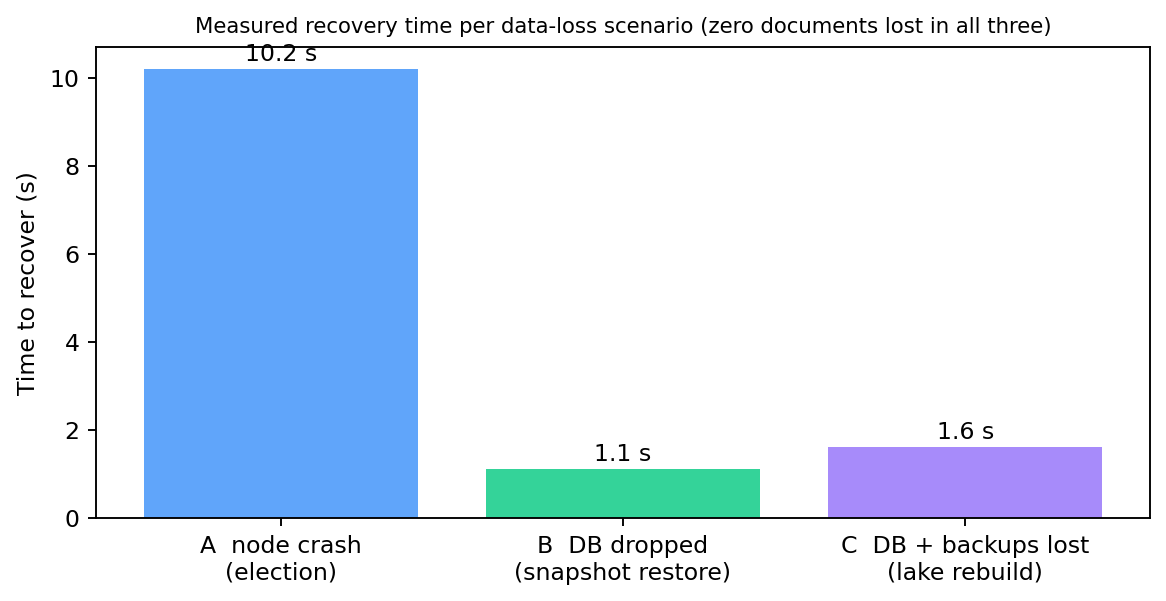
\includegraphics[width=0.75\textwidth]{images/StoryIndex.png}
\caption{Measured recovery time per scenario}
\label{fig:rec}
\end{figure}

\paragraph{Recovery objectives.} Recovery point (RPO): up to the backup interval for scenario B (24\,h with a daily schedule); 0 events for scenario C because the lake is written in the same micro-batch as MongoDB. Recovery time (RTO): about 1 to 2\,s at demo scale; it grows with data volume. \textbf{What scenario C cannot restore:} the per-rule reason text of an alert (the lake stores rule and ML verdicts, so recovered alerts say \texttt{RULE\_ALERT} or \texttt{ML\_PAYLOAD\_ANOMALY}), original batch timestamps and malformed-record counts. \textbf{Not covered:} backups and lake share one disk with the database, so loss of the machine is not survived without an off-site copy.

\section{Sharding}
\paragraph{}
Hashing the \texttt{\_id} divided 377,325 alerts into 188,683 and 188,642 documents (maximum/minimum ratio 1.0). A lookup by \texttt{\_id} contacted one shard; a filter on \texttt{run\_id} contacted both, the expected scatter-gather cost of choosing \texttt{\_id} as the key. Both shards share one laptop, so this demonstrates distribution, routing and failover, not a throughput gain.

\section{Detection quality}
\begin{table}[H]
\centering
\begin{tabular}{|l|c|c|c|c|}
\hline
\textbf{Full run, 1,410,255 records} & \textbf{Precision} & \textbf{Recall} & \textbf{F1} & \textbf{FPR} \\ \hline
Baseline metadata rules & 98.28\% & 67.67\% & 80.15\% & 3.43\% \\ \hline
Hybrid (rules OR MLlib) & 98.25\% & 99.85\% & 99.04\% & 5.15\% \\ \hline
\end{tabular}
\caption{Detection results on the complete dataset (hybrid: TP 1,046,576; FP 18,652; TN 343,456; FN 1,571)}
\end{table}

\paragraph{}
The payload model removed 337,272 of the 338,843 missed attacks. Figure~\ref{DP2} shows the gain by attack family on a held-out split of a 10,000-row sample: families that the metadata rules miss completely (Infiltration, Web brute force, XSS, Bot) are detected by the payload model. The price is a higher false-positive rate (3.43\% to 5.15\%) because the rule and ML alerts are united.

\begin{figure}[H]
\centering
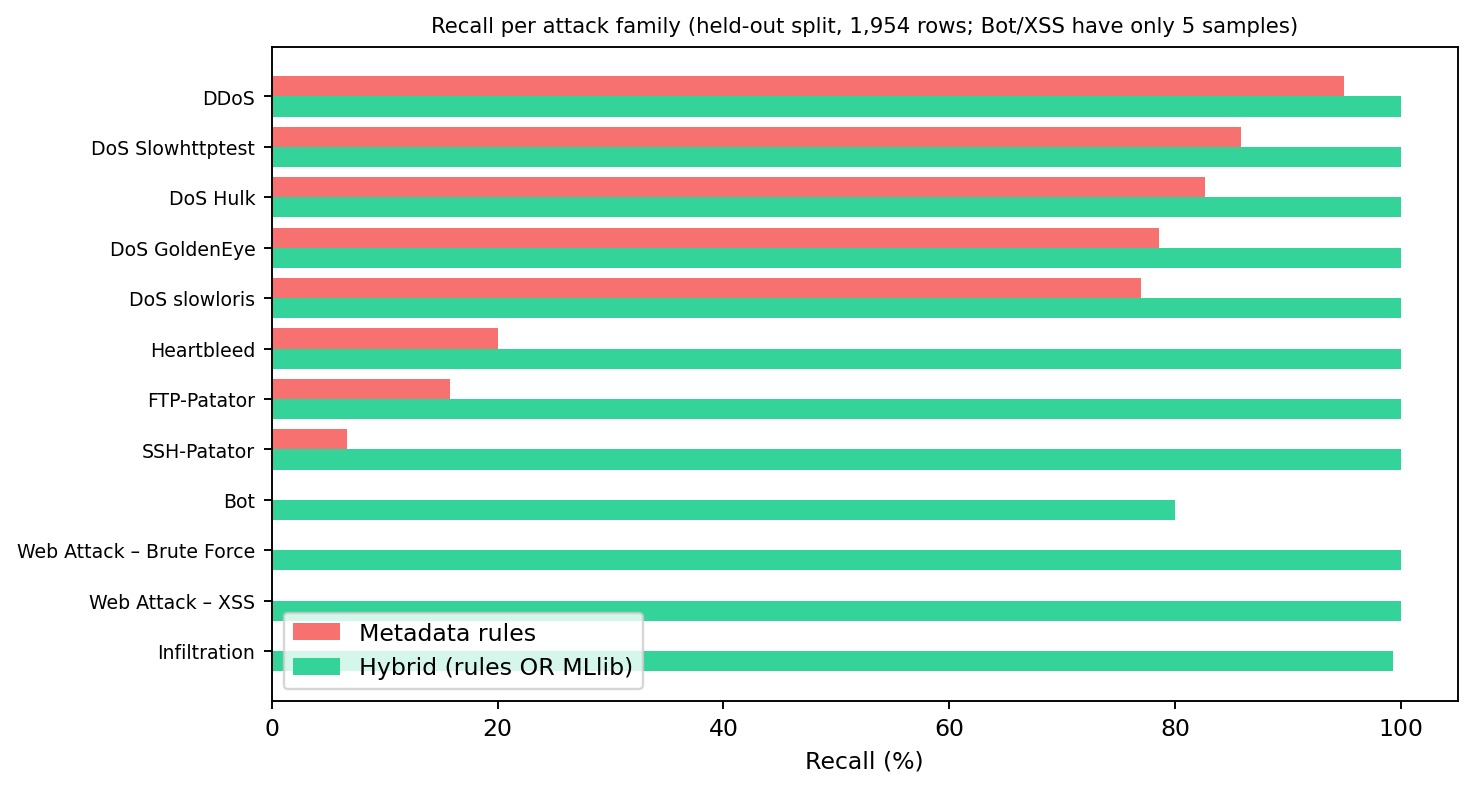
\includegraphics[width=0.85\textwidth]{images/DP2.png}
\caption{Recall per attack family: metadata rules versus hybrid}
\label{DP2}
\end{figure}

\paragraph{Caveats.} PCA with 32 components explains 74.2\% of the payload variance (128 components: 81.9\%, with no gain in F1), so 95\% variance is not reached; the model was trained on a 10,000-row sample that overlaps the full run by about 0.6\%; and CIC-IDS2017 attacks are very separable, so results on live traffic would be lower. On the offline split ML alone had the best F1 (99.62\%, FPR 1.79\%) against 99.04\% for the hybrid (FPR 5.16\%); the hybrid is preferable when missing a volumetric attack is costlier than a false alarm.

\section{Throughput and storage}
\paragraph{}
Ingesting 420,000 metadata records with the lake dual write, Spark reached 9,635 records/s from a one-partition topic and 12,889 records/s from a four-partition topic (+34\%). The 20,000 records/s target was \textbf{not} reached on this machine; the benchmark ran with the cluster, Kafka and Spark sharing 7.5\,GB of RAM. The complete 1.41 million-record run with payloads, lake and hybrid detector finished with 100\% of records processed. The lake held the full run in 43\,MB, and Parquet was 3.98$\times$ smaller and about 11$\times$ faster to scan than CSV.

\section{Dashboard}
\paragraph{}
Figures of the original dashboard are in Appendix~A. The extended dashboard adds two tabs: \emph{Batch Lake Analytics} (tumbling versus sliding window alerts, protocol table, payload-entropy histogram, attack-family detection, TTL heat map, CSV versus Parquet study) and \emph{System Health \& Disaster Recovery} (last backup and its verification state, lake size, Kafka consumer lag per partition, and the role and health of each node in each shard).
